\documentclass{article}

% if you need to pass options to natbib, use, e.g.:
% \PassOptionsToPackage{numbers, compress}{natbib}
% before loading nips_2018

% ready for submission
% \usepackage{nips_2018}

% to compile a preprint version, e.g., for submission to arXiv, add
% add the [preprint] option:
% \usepackage[preprint]{nips_2018}

% to compile a camera-ready version, add the [final] option, e.g.:
\usepackage[final]{sos_final}

% to avoid loading the natbib package, add option nonatbib:
% \usepackage[nonatbib]{nips_2018}

\usepackage[utf8]{inputenc} % allow utf-8 input
\usepackage[T1]{fontenc}    % use 8-bit T1 fonts
\usepackage{hyperref}       % hyperlinks
\usepackage{url}            % simple URL typesetting
\usepackage{booktabs}       % professional-quality tables
\usepackage{amsfonts}       % blackboard math symbols
\usepackage{nicefrac}       % compact symbols for 1/2, etc.
\usepackage{microtype}      % microtypography
\usepackage{amsmath}
\usepackage{graphicx}
\usepackage{float}

\title{Sum of Squares Solver for Python}

\author{
  Allen Kim \\
  PhD, Computer Science\\
  Stony Brook University\\
  \texttt{allen.kim@stonybrook.edu} \\
}

\begin{document}
% \nipsfinalcopy is no longer used

\maketitle

\begin{abstract}
    We implement a sum of squares tester for arbitrary polynomials in Python found in \url{https://github.com/allenkim/sos-solver} . Sum of squares analysis has been increasingly important for numerous areas in optimization and control as it provides a tractable framework for computations. Trying to determine non-negativity or convexity in general is NP hard, so sum of squares provides a practical alternative. However, as it is a relatively new area, most implementations are in MATLAB. We discuss the algorithms used to test feasibility of sum of squares, its implementation in Python, and other potential applications this leads to.
\end{abstract}

\section{Background}

For the purposes of many practical applications, it is often important to know when functions are convex or non-negative. Unfortunately, even when restricting ourselves to polynomials, determining whether a polynomial is non-negative or convex is NP-hard for polynomials with degree as small as four.. However, an alternative to these notions were considered: sum of squares representation. In general, this acts as a tractable substitute for non-negativity.

We first consider some definitions. Formally, we say that a polynomial $p(x)$ is said to be nonnegative or positive semidefinite if \[p(x) \ge 0\] 
for all $x \in \mathbb{R}^n$. We also say that a
polynomial $p(x)$ is a sum of squares (SOS) if it can be represented as a sum of square polynomials, meaning that there exists polynomials $q_1(x),\ldots,q_m(x)$ such that \[p(x) = \sum_{i=1}^m q_i^2(x)\]

It is clear that if a polynomial is SOS, then it is nonnegative. However, the converse is not necessarily true in general. It was shown by Hilbert that this is only true for for univariate, quadratic, and bivariate quartics, but not true in all other cases \cite{sos_convex}. The classic example is Motzkin's polynomial:
\[f(x,y) = 1 + x^4y^2 + x^2y^4 - 3x^2y^2\]
This function can be shown to be non-negative by the arithmetic-geometric inequality as follows:
\[\frac{1+x^4y^2 + x^2y^4}{3} \ge (1 \cdot x^4y^2 \cdot x^2y^4)^\frac{1}{3}\]
It was also proven that it cannot be represented as a sum of squares through algebraic manipulation, which we will not go into here, but can be found at \cite{hilbert}.

\section{Setup}

Currently, the main implementations relating to sum of square solvers are in MATLAB \cite{sostools}, but there are no well-known ones in Python. Thus, we aimed to port some functionality of the sum of squares solvers in MATLAB to Python using the algorithms described in their papers.

To mimic the symbolic manipulations of variables in MATLAB, we used SymPy. This enabled us to work directly with polynomial expressions. Additionally, we used NumPy for functions related to linear algebra and CVXPY for solving semidefinite programs. The exact way in which these libraries were used is discussed in detail in the next section.

\section{Algorithm Overview}

For our project, we aim to determine whether a given polynomial yields a sum of
squares decomposition algorithmically. We outline the steps in the following subsections.

\subsection{Initializing Polynomial}

We first use SymPy to initialize the polynomials. Below is an example of how one would set up the polynomials they want to check.

\begin{verbatim}
syms = symbols('x y')
x, y = syms
poly = 2*x**4 + 2*x**3*y - x**2y**2 + 5*y**4
\end{verbatim}

\subsection{Converting to Semidefinite Program}
We first have to convert the given polynomial as a feasibility problem using
semidefinite programming. An important theorem tells us that a multivariate polynomial $p(x)$ in $n$
variables and degree $2d$ is a sum of squares if and only if there exists a
positive semidefinite matrix $Q$ such that $$p(x) = z^T Q z$$ where $z$ is the
vector of monomials of degree up to $d$ \cite{sos_convex}$$z = [1,x_1,x_2,\ldots,x_n, x_1x_2,
\ldots, x_n^d]$$ 

One point to note is the number of possible monomials is $n+d \choose d$. However, if the polynomial is homogeneous, meaning that the degree of each monomial in the polynomial is equal, then we only need to consider monomials of degree exactly $d$ \cite{sos_convex}. In that case, the number of possible monomials become $n+d-1 \choose d$. These values for the number of possible monomials come from a combinatorial argument using stars and bars.

Given the coefficients of $p$, we can expand $z^TQz$ and match the coefficients to  get linear constraints on $Q$. If we let $q$ be the vectors of $Q$ stacked on top of each other vertically, we can represent these linear constraints as $Aq = b$. \cite{sosopt} Thus, we get the SDP:
\begin{center}
	Given a matrix $A$ and vector $b$, find $Q \ge 0$ such that $Aq=b$.
\end{center}

As an example, we had $p(x,y) = 2x^4 + 2x^3y - x^2y^2 + 5y^4$. Thus, we can get the following expansion:
\begin{align*}
p(x,y) &= 2x^4 + 2x^3y - x^2y^2 + 5y^4\\
&= \begin{bmatrix}
x^2 \\
xy \\
y^2
\end{bmatrix}^T
\begin{bmatrix}
q_0 & q_1 & q_2 \\
q_3 & q_4 & q_5 \\
q_6 & q_7 & q_8
\end{bmatrix}
\begin{bmatrix}
x^2 \\
xy \\
y^2
\end{bmatrix}\\
&= q_0x^4 + (q_1+q_3)x^3y + (q_2+q_4+q_6)x^2y^2 + (q_5+q_7)xy^3 + q_8y^4
\end{align*}

We also know that $Q$ must be symmetric, so we get the following equality constraints:
\begin{align*}
q_0 &= 2 & q_1+q_3 &= 2 & q_2+q_4+q_6 &= -1 & q_5+q_7 &= 0 & q_8 = 5
\end{align*}
\begin{align*}
q_1 &= q_3 & q_2 &= q_6 & q_5 &= q_7
\end{align*}

This conversion was done purely with SymPy for the symbolic manipulations and NumPy for the matrix operations.

\subsection{Solving Semidefinite Program}
We now have to find a positive semidefinite $Q$ that satisfies the given linear constraints. In general, these problems are solved using interior point methods \cite{sdp}. Since there were already many implementations of these methods available already, we decided to use one called CVXPY that solves these semidefinite programs for us.

We note that this is not exactly an optimization problem since there is no value we are optimizing. This is a feasibility problem, so we need not care about minimizing any value and can just consider a constant instead.

Also, note that $Q$ is not unique, so there is more than one way to convert a polynomial to a sum of squares representation. For the running example, we can find one such $Q$:

\[Q = \begin{bmatrix}
2.   &       1.    &     -1.05645373 \\
1.   &       1.11290746 & 0.        \\
-1.05645373 & 0.     &     5.        
\end{bmatrix}
\]

\subsection{Converting back to Sum of Squares}
We then have to convert the solution to the SDP back into a sum of squares (if one exists).

Once we have a $Q$, since $Q$ is a PSD matrix, we can compute its Cholesky
decomposition to get $Q = V^TV$ and then, output the sum of squares
directly \cite{sos_convex}: $$p(x) = z^TQz = z^TV^TVz = \sum_i (Vz)_i^2$$

We note that there is actually a issue that arises when $Q$ turns out to have zero eigenvalues. Cholesky decomposition only works on just positive definite matrices, so in the case there are zero eigenvalues, we add some $\epsilon$ to the diagonal matrix. By perturbing the diagonal slightly, we can make $Q$ purely positive definite.

For the running example, we can decompose $Q$ to $V^TV$, where:
\[V = \begin{bmatrix}
1.41421356 & 0.70710678 & -0.7470256 \\
0.         & 0.78288407 &  0.67471914 \\
0.         & 0.         &  1.99667394 
\end{bmatrix}\]

By multiplying with our vector of monomials $z$, we get our final sum of squares representation:

\begin{verbatim}
p(x,y) = 3.98670683710615*y**4 + 
(0.782884066722985*x*y + 0.674719141613451*y**2)**2 + 
(1.41421356237309*x**2 + 0.707106781186547*x*y - 0.747025597174727*y**2)**2
\end{verbatim}

As mentioned before, $Q$ is not unique and thus, there can be multiple representations such as this one:
\[p(x,y) = \frac{1}{2}(2x^2-3y^2+xy)^2 + \frac{1}{2}(y^2+3xy)^2\]

Thus, we see that our original polynomial $p(x,y) = 2x^4 + 2x^3y - x^2y^2 + 5y^4$ was non-negative.

\section{Applications}

One nice application for this method is to find minimums of polynomials. The main idea is to consider the following optimization problem \cite{Parrilo03minimizingpolynomial}:
\begin{align*}
\max \gamma \text{ such that } \\
p(x)-\gamma \ge 0
\end{align*}

We see that the main idea is to subtract as large a value as possible from a polynomial while still maintaining semi-positivity. One nice aspect of this approach is that it does not matter whether the polynomial is convex or not. Typically, many minimizing techniques rely on the convexity of the function, but in this case, no such assumptions are made. However, this only guarantees a lower bound, and not necessarily the exact minimum. However, it turns out that it can find the exact minimum in many cases. 

We added this functionality by converting the feasibility problem from before into an optimization problem over $\gamma$. We discuss some examples and results below.

One example is this function:
\[f(x,y) = 4x^2 - \frac{21}{10}x^4 + \frac{1}{3}x^6 + xy - 4y^2 + 4y^4\]

\begin{figure}
	\centering
	\begin{minipage}{0.45\textwidth}
		\centering
		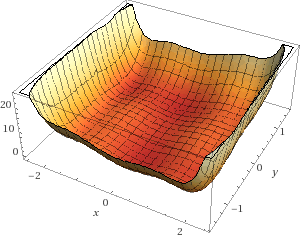
\includegraphics[width=0.9\textwidth]{plot1}
		\caption{3D Plot of $f(x,y)$}
	\end{minipage}\hfill
	\begin{minipage}{0.45\textwidth}
		\centering
		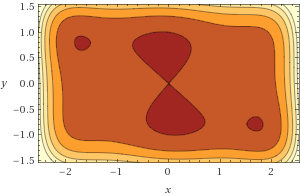
\includegraphics[width=0.9\textwidth]{plot2} % second figure itself
		\caption{Contour plots of $f(x,y)$}
	\end{minipage}
\end{figure}

This function is clearly not convex as it has four separate minimums as shown in Figures 1 and 2. After running our optimizer, we found that the minimum value was $-1.0316313547159408$, which turns out to be the actual minimum of the function. This was found in about 0.4 seconds.


We also have the Goldstein Price function that we wanted to test on, which is given as:
\begin{align*}
f(x,y)=[1 + (x + y + 1)^2(19 - 14x+3x^2 - 14y + 6xy + 3y^2)]\\
[30 + (2x - 3y)^2(18 - 32x + 12x^2 + 4y- 36xy + 27y^2)]
\end{align*}

\begin{figure}[H]
	\centering
	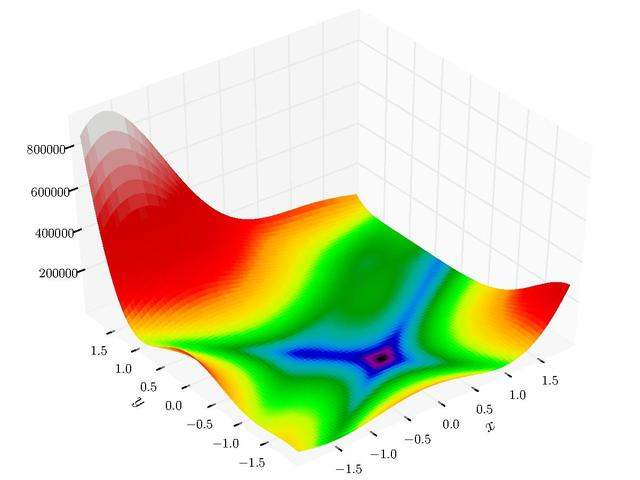
\includegraphics[scale=1]{goldstein} 
	\caption{Goldstein Price Function \cite{goldstein}}
\end{figure}

Figure 3 shows the plot of this function. We see that this function is not convex and has a lot of irregularities. After running the optimizer, we found a value of 3.000942899362592, which is close to the actual minimum of 3 (most likely due to floating point precision). This was found in about 2.2 seconds.

\section{Future Work and Conclusion}

There are many venues of expanding this project which we did not yet do. For the sum of squares decomposition, we note that everything was done with floating point numbers, but this may not be ideal for applications that require exact answers. For these cases, rational numbers would be better suited. By sticking with rational numbers, none of the precision is lost and the final answer can be represented exactly with fractional coefficients.

Another important feature would be to actually find the point that minimizes or lower bounds the polynomials. In the applications, we find a minimal value itself, but not the point that evaluates to it. This could be done by considering appropriate primal and dual semidefinite programs as found in \cite{Parrilo03minimizingpolynomial}.

In the end, we implemented a simple sum of squares checker as well as a lower bound evaluator for arbitrary polynomials in Python. This was done using SymPy for symbolic manipulation, NumPy for matrix operations, and CVXPY for solving the SDP.


\bibliographystyle{unsrt}
\bibliography{sos_final}

\end{document}

